% =====================================================================
% Слайд 7 — Baseline 2: HMM (наработка лаборатории)
% =====================================================================
\begin{frame}{Baseline 2: HMM \small(Rabiner 1989)}
  \footnotesize\setlength{\abovedisplayskip}{3pt}
  \setlength{\belowdisplayskip}{3pt}

  Скрытая Марковская модель по партитуре.

  \begin{columns}[T,onlytextwidth]
    \column{0.50\textwidth}
    \vspace{0.4em}
    \begin{itemize}\setlength{\itemsep}{0.35em}
      \item Состояния: $i \in \{0,\ldots,N{-}1\}$ --- индексы нот.
      \item Эмиссия (гауссиана по pitch, $\sigma$ в полутонах):
            \[
              b_i(o) = \frac{1}{\sigma\sqrt{2\pi}}
              \exp\!\Bigl(-\tfrac12
              \bigl(\tfrac{o - p_i}{\sigma}\bigr)^{\!2}\Bigr)
            \]
      \item Переходы $\{$stay$=0.3$, advance$=0.6$, skip$=0.1\}$,
            веса зависят от \texttt{elapsed} в state.
      \item Forward-обновление:
            \[
              \alpha_{t+1}(i) = b_i(o_{t+1}) \sum_j \alpha_t(j)\, a_{j,i}
            \]
      \item $\hat\imath_t = \argmax_i \alpha_t(i)$,\quad
            \emph{confidence} $= \max_i \alpha_t(i)$.
    \end{itemize}

    \column{0.50\textwidth}
    \centering
    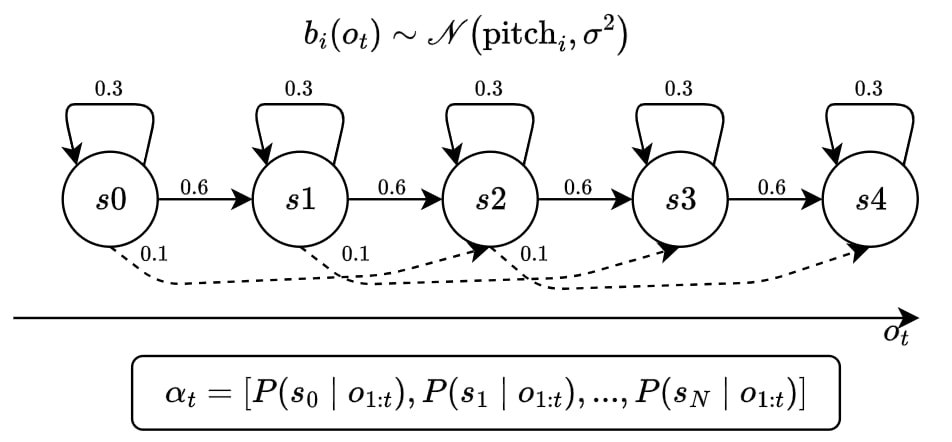
\includegraphics[width=\linewidth]{figures/png/hmm_chain.png}
  \end{columns}
\end{frame}
